\chapter{DATA C100: Constant Model}

\section{Defining the Constant Model}
Now that we have finished reading about simple linear regression from the previous lecture, let us discuss a slightly simpler model.
\begin{ln-define}{Constant Model}{}
    \textbf{Constant Model}, also known as a summary statistic, summarizes the sample data by always predicting the same number for any data point. \\
    Mathematically expressed,
    \[\hat{y} = \theta\]
\end{ln-define}
In other words, the estimated $y$ is always a constant parameter $\theta$, whatever the input might be.

\section{Experimenting Different Loss Functions}
A model may have several options for its loss functions, which comes with different advantages and disadvantages. \\
For this constant model, let us explore the L2 and L1 loss functions, see how each brings a different condition of optimization and robustness.

\subsection{Exploring L2 Loss: MSE}
In the L2 case, let us recall that our empirical risk is defined as follows:
\[R(\theta) = \frac{1}{n} \sum_{i = 1}^n {(y_i - \hat{y}_i)}^2\]
Therefore, for our constant model:
\[R(\theta) = \frac{1}{n} \sum_{i = 1}^n {(y_i - \theta)}^2\]
Let us proceed onto its optimization by attempting to find the critical point of empirical risk:
\begin{ln-derive}{Optimization of L2 Empirical Risk for Constant Model}{}
    \begin{align*}
        \pdv{R}{\theta}
        &= \frac{1}{n} \sum_{i = 1}^n 2\frac{\delta}{\delta \theta}(y_i - \theta){(y_i - \theta)} \\
        &= -\frac{2}{n} \sum_{i = 1}^n (y_i - \theta)
    \end{align*}
    And now, to optimize $R$,
    \begin{align*}
        \sum_{i = 1}^n (y_i - \theta) &= 0 \\
        \overline{y} - \theta &= 0 \\
        \theta = \overline{y}
    \end{align*}
    Therefore, 
    \[\hat{\theta} = \overline{y}\]
\end{ln-derive}
Let us enjoy some observations here. \\
First of all, the minimum MSE is thus:
\[R(\theta) = \frac{1}{n} \sum_{i = 1}^n {(y_i - \overline{y})}^2 = \sigma_y^2\]
, the variance of $y$. \\
Second of all, the estimated value of parameter $\theta$ is thus the mean of $y$. This means, provided an extreme outlier, the model will misbehave due to the mean being heavily influenced by some extreme outlier(s). Therefore, L2 Loss is not very robust (adaptative) towards the appearance of outliers. \\

\subsection{Exploring L1 Loss: MAE}
The L1 Loss Empirical Risk is also known as \textbf{Mean Absolute Difference}, which followed a similar naming logic to MSE. \\
Mathematically expressed,
\[R(\theta) = \frac{1}{n} \sum_{i = 1}^n |(y_i - \theta)|\]
The optimization of such an empirical risk becomes interesting (matheamtically), due to the appearance of absolute value. \\
However, we may always characterize the absolute value as a piecewise function:
\[
    f(x) = |x - \theta|
    \rightarrow
    f(x) = 
    \begin{cases}
        x - \theta, &x > \theta \\
        0, &x = \theta \\
        \theta - x, &x < \theta
    \end{cases}
\]
Let us exploit this in the following toil:
\begin{ln-derive}{Optimization of L2 Empirical Risk for Constant Model}{}
    \[
        |y_i - \theta|
         = 
        \begin{cases}
            y_i - \theta, &y_i > \theta \\
            0, &y_i = \theta \\
            \theta - y_i, &y_i < \theta
        \end{cases}
    \]
    \[
        \frac{\delta}{\delta \theta}|y_i - \theta|
        = 
        \begin{cases}
            1, &y_i > \theta \\
            0, &y_i = \theta \\
            -1, &y_i < \theta
        \end{cases}
    \]
    \begin{align*}
        \pdv{R}{\theta}
        &= \frac{1}{n} (\sum_{\theta < y_i}(-1) + \sum_{\theta > y_i}(1)) \\
        \sum_{\theta < y_i}(-1) + \sum_{\theta > y_i}(1) &= 0 \\
        \sum_{\theta > y_i}(1) = \sum_{\theta < y_i}(1)
    \end{align*}
    Therefore, $\hat{\theta}$ must be the median of $y$.
\end{ln-derive}
The estimated value of parameter $\theta$ is thus the mean of $y$. This means, provided an extreme outlier, the model will not misbehave due to the median not easily influenced by some extreme outlier(s). Therefore, L1 Loss is more robust (adaptative) towards the appearance of outliers. \\

\subsection{Summary of Loss Function Optimization}
In summary, the process of finding optimization conditions (which we also call \textbf{estimating equation}) would follow:
\begin{enumerate}
    \item Differentiate the empirical risk with respect to parameters.
    \item Attempt to find the critical point of empirical risk for per parameter.
    \item Perform the derivative test (which requires multivariable calculus in most occassions, and is not performed for the span of DATA C100 for that reason) to confirm that the critical point is a minima.
\end{enumerate}
The multivariable perspective offers a much computationally heavy test for confirming whether a critical point is a minima, which would involve calculating plural higher order partial derivatives. For those who are interested, this is in-scope for MATH 53.

\section{Transformation and Model Linearity}
In some cases, we face how the predictor variable $x$ is not linearly correlated with $y$, but a transformation of $x$ might be. \\
For example, the trajectory of a baseball is mostly quadratic. If I'd like to predict its motion, it is best that I present a model whose shape is not linear, but rather, quadratic:
\[\hat{y} = \hat{a} + \hat{b} x^2 \]
This happens frequently across datasets, but the question is: is the model still linear in this case? \\
The answer is yes. Linear Regression requires a regression line, decided as a linear combination of parameters. In this case, the predictor variable is being a non-linear term, but the regression equation is still linear with respect to each of the parameters.

As previously mentioned, models sometimes require transformations to behave better, fitting to the behaviour of the dataset more closely. \\
To decide what transformations seem optimal, we can employ the following figure:
\begin{ln-fig}{Turkey-Mosteller Bulging Diagram}{}
    \begin{center}
        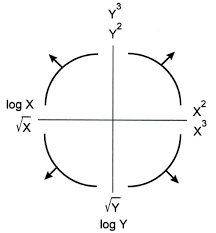
\includegraphics[scale=0.8]{figs/ln02/turkey-mosteller.png}
    \end{center}
\end{ln-fig}
Each of these transformations suggest how to transform $x$ and $y$ via suggesting that, for the direction that data's shape currently bulges towards, we should transform $x$ and/or $y$ in that direction. \\
In this case, we are usually then given the choice to either transform $x$ or $y$, or as priorly mentioned, perhaps both.
